\chapter{Modelling of electrokinetic flow}\label{sec:res}
In this chapter, results of modelling of electrokinetic flow using the
previously described lattice-Boltzmann method are presented. The
choice of systems is done with focus on those where the
Poisson-Boltzmann approach is not applicable. First simple 1D systems
in channels are considered, then more complicated systems in 2D. All
results presented here are for systems in steady state. The liquid
used in the modelling is a KCl solution defined by the parameters in
tab. \ref{tab:res:param}.

\begin{table}
  \caption{Physical parameters of the KCl ion solution that is modelled
    in this chapter. Parameters are from \cite{dongquing-ren-book}. }
\begin{center}
    \begin{tabular}{ | r | l |}
    \hline
    Relative permittivity, $\ep_r$ & 80\\
    Mean ionic conentration, $\cnil$ & $10^{-4}$ mol/m$^3$\\
    Conductivity, $\sigma_c$ & 1.5 mS/m\\
    Temperature, T & 293 K\\
    kinematic viscosity, $\nu$ & 1.0 $\mu$m$^2$/s\\
    Diffusion coefficient, $D_+ = D_{-}$ & $ 10^{-10}$ m$^2$/s\\
    \hline
    \end{tabular}
\end{center}    
\label{tab:res:param}
\end{table}

\section{Charge concentration and potential in 1D system}
To get a feeling for the systems dealt with here, a system where no
advection is present is first be considered. The geometry consists
of a 2D channel where both walls are negatively charged. As earlier
discussed in chapter \ref{sec:et}, positive ions will be attracted to
the walls and negative will be repelled.

A channel of width $10 \mu$m and with walls with a surface charge of
$3.5 \mu$C/m is considered. The computed electric potential in the
steady state for this system is presented in
fig. \ref{fig:res:pot_1d}. With the particular choice of width and
surface charge, we see that the double layers extend a substantial
length into the channel. The Debye length is in this case $\kappa^{-1} =
1 \mu$m and $d\kappa = 10$. It is the charcteristic EDL length that
is compared with when stating that a channel is wide or
narrow. If $d\kappa \gg 1$, the channel is said to be wide otherwise
narrow. In this section mainly narrow channels are studied.

\begin{figure}
\begin{center}
\includegraphics[width=0.9\textwidth]{fig/potential_1d.pdf}
\end{center}
\caption[Computed electric potential across a channel.]{Computed
  electric potential across a channel of width $d = 10 \mu$m. The
  solution in the channel is a KCl solution defined by parameters in
  table \ref{tab:res:param}. The channel walls are negatively
  charged. Note that $\Vnil$ is negative.}
\label{fig:res:pot_1d}
\end{figure}

Also the concentrations of positive and negative ions corresponding to
the potential are visualised in fig. \ref{fig:res:c_1d}. The surplus
of positive ions in the vicinity of the walls together with the
surplus of negative ions at the centre of the channel are clearly shown. 

\begin{figure}
\begin{center}
\includegraphics[width=0.9\textwidth]{fig/charge_1d.pdf}
\end{center}
\caption[Computed positive and negative charge distributions across a
  channel]{Computed positive (solid) and negative (dashed) charge
  distribution across a channel of width $d = 10 \mu$m. The solution
  in the channel is a KCl solution defined by parameters in table
  \ref{tab:res:param}. The channel walls are negatively charged.}
\label{fig:res:c_1d}
\end{figure}

\subsection{Nernst-Planck vs. Poisson-Boltzmann}
In the Poisson-Boltzmann model, section \ref{sec:et:pb}, the parameter
$\C_i^{\infty}$ that determines the value of the concentration far
from the EDL is chosen as the bulk concentration of the fluid. The
problem with narrow channels is that there is no bulk and as we see in
fig. \ref{fig:res:c_1d}, it would not be an accurate choice. Also if
$\C_i^{\infty}$ would be set to the bulk concentration for a narrow
channel the total number of ions would not be preserved. For a 1:1
solution and with negatively charged channel walls, the number of
positive ions would not equal the number of negative ions.

Further assumptions made in the Poisson-Boltzmann model is that of a
simple geometry, the thickness of the EDL must be small to the
curvature of the boundary. Also no advection is assumed. 




\section{Electroviscous effect}
In section \ref{sec:et:streaming_pot}, the physical model behind
pressure-driven electrokinetic flow is presented. The effect of
interest that arise in this kind of systems is the electroviscous
effect.

Velocity profiles computed in a 1D situation is presented here. We
consider a 1 $\mu$m wide channel that has negatively charged
walls. The wall charge is a parameter that is varied and from this the
effect on the velocity profile is studied. The system is setup with a
Peclet number, $\Pe = 1$ and a Reynolds number, $\Rerm = 10^{-4}$. To
drive the flow, a pressure gradient of 1 kPa/m is set. The resulting
velocity profiles are presented in fig. \ref{fig:res:ev}.

\begin{figure}
\begin{center}
\includegraphics[width=0.9\textwidth]{fig/electrovisc.pdf}
\end{center}
\caption[Computed velocity profiles, illustrating the electroviscous
  effect.]{Computed velocity profiles across a 2D channel of width $d
  = 1 \mu$m. The flow is driven by a pressure gradient and the flow is
  slowed down due to the electroviscouos effect, this effects
  dependence on the surface charge $\sigma_s$ is here illustrated. The
  solution in the channel is a KCl solution defined by parameters in
  table \ref{tab:res:param}. In this simulation, $\sigma_0 = 0.89
  \mu$C/m$^2$, $\partial_xP = 1$ kPa/m and $u_0 = 10$ mm/s. }
\label{fig:res:ev}
\end{figure}

The velocity profiles obtained agrees qualitatively with a similar
simulation preformed in \cite{ren-elvis-paper}. The local minimum that
arises for $\sigma_s  = 20\sigma_0$ is due the high accumulation of
negative ions in the middle of the channel. This is an effect that
only is seen for narrow channels.

In the model proposed here, using Ohm's law to relate the ion current
to the streaming potential, the force on the flow due to the
electroviscous effect is opposite to the flow everywhere where there
is a net charge present in the fluid. However, in most texts about the
electroviscous effect, e.g. in \cite{dongquing-ren-book},
\cite{wang-poi} and \cite{ren-elvis-paper}, this force is computed
using a mean current approach. An integration of ion flux over the
cross-section of the channel is performed and then a net current for
the whole channel is obtained. From this current, a mean streaming
potential is obtained for the channel and a force is calculated using
the charge density. This gives that positive and negative net charged
regions of the fluid will be affected with forces of opposite sign
respectively. Having a mean streaming potential for the whole channel
also gives contraintuitve results when considering the fact that
regions in the fluid with the same net charge but different velocities
is affected by the same force. Also with this approach the
electroviscous effect would in principle be able to locally oppose the
flow direction. Also, in a more complicated geometry, this approach
would break down. In fig. \ref{fig:res:ev_comp}, two velocity profiles
from fig. \ref{fig:res:ev} are compared with corresponding profiles
computed using the mean current approach. It is seen that the
force slowing down flow is smaller for the case when using a mean
current. This is due to the cancellation between negative and
positive ion fluxes in the integration.

\begin{figure}
\begin{center}
\includegraphics[width=0.9\textwidth]{fig/electrovisc_comp.pdf}
\end{center}
\caption[Comparison between electroviscous flow using the traditional
  and local approach.]{Comparison between velocity profiles computed
  using a mean current (dotted) and by using the actual local current
  (dashed) for the streaming potential. The solution in the channel is
  a KCl solution defined by parameters in table
  \ref{tab:res:param}. In this simulation, $\sigma_0 = 0.89
  \mu$C/m$^2$, $\partial_xP = 1$ kPa/m and $u_0 = 10$ mm/s. }
\label{fig:res:ev_comp}
\end{figure}


\section{Electroosmotic flow}
As described in section \ref{sec:et:electroosmosis}, electroosmotic
flow is driven by an electric field rather than a pressure gradient.
Charge particles will be affected by a force and will drag the fluid
with them. The effect is investigated in this section.

A 10 $\mu$m channel is considered with walls charged with $3.56
\mu$C/m$^2$. The 1:1 ratio between positive and negative ions is in
this section put aside for a moment. To investigate how the
electroosmotic flow behaves for different situations of the charge
density, especially in the middle of the channel, the amount of
negative ions are varied. The different situations are investigated, a
surplus and a lack of negative ions together with a neutral solution
at the middle of the channel. Thus, the following values of the mean
concentration of negative ions are set: $0.7\C_0$, $0.75\C_0$,
$0.78\C_0$, $0.8\C_0$ and $0.85\C_0$. 

A constant electric field of $10^5$ V/m along the channel are set
and the same Peclet and Reynolds number as before are used. The
obtained ion concentrations and the velocity profiles are presented in
fig. \ref{fig:res:eo_charge} and fig. \ref{fig:res:eo_u}
respectively. 

\begin{figure}
\begin{center}
\includegraphics[width=0.9\textwidth]{fig/eo_conc.pdf}
\end{center}
\caption[Charge distributions for a varied ratio of positive and
  negative ions.]{Computed charge distributions for positive (solid)
  and negative (dashed) ions. The mean concentration of positive ions
  is $\C_0$ while that of negative ions are varied between the values
  $0.7\C_0$, $0.75\C_0$, $0.78\C_0$, $0.8\C_0$ and $0.85\C_0$. The
  geometry is a channel of width $10 \mu$m.}
\label{fig:res:eo_charge}
\end{figure}

\begin{figure}
\begin{center}
\includegraphics[width=0.9\textwidth]{fig/eo_u.pdf}
\end{center}
\caption[Computed velocity profiles for electroosmotic flow.]{Computed
  velocity profiles for electroosmotic flow, in a $10 \mu$m wide
  channel. The different profiles correspond to different ratios
  between positive and negative ions, see
  fig. \ref{fig:res:eo_charge}. The solid profile is the ``plug flow''
  that corresponds to the Poisson-Boltzmann case, where the middle of
  the channel is net neutrally charged.}
\label{fig:res:eo_u}
\end{figure}

In the case with a neutral middle of the channel the traditional
``plug profile'' of electroosmotic flow for wide channels are
reproduced. In this case the force from the electric field only
affects the fluid near the walls where a net charge is present, due to
viscous forces, a constant velocity profile is then obtained in the
middle of the channel. For a positive net charge in the middle of the
channel and thereby everywhere in the channel, the velocity profiles
are not of the ``plug'' shape but more parabolic. For a negatively net
charged middle of the channel and with the parameter of choice, the
viscous effect only compensates for the opposing effect from the
electric field when there is a small negative net charge. We see that
in this case, with the chosen parameters, for a 1:1 solution the flow
would be completely opposite of the electric field which is an
apparent difference to the wide channel case.


\section{Flow in a channel with heterogeneously charged walls}

Now a channel with walls charged with a varying charge is
considered. The walls are charged piecewise constant with every second
piece positive and negative respectively, see
fig. \ref{fig:res:h_setup}. The length of the charged sections are
chosen as $d/4$ where $d = 10 \mu$m is the width of the channel. The
flow is electroosmotic and driven by an external field of $50$ kV/m.

\begin{figure}
  \centering
  \subfloat[Heterogeneous wall charge
    ]{\label{fig:res:h_setup}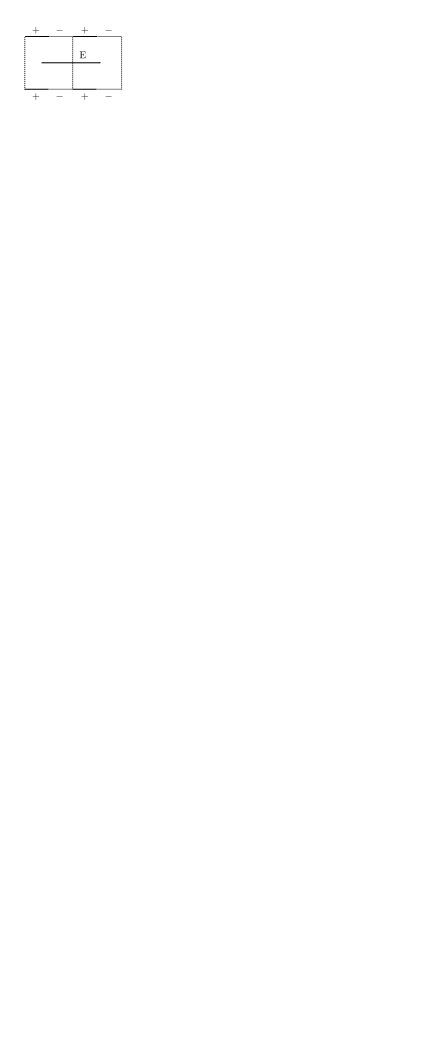
\includegraphics[width=0.35\textwidth]{fig/hetro_setup.pdf}}      
  \hspace{5pt} \subfloat[Array of charged squares
  ]{\label{fig:res:square}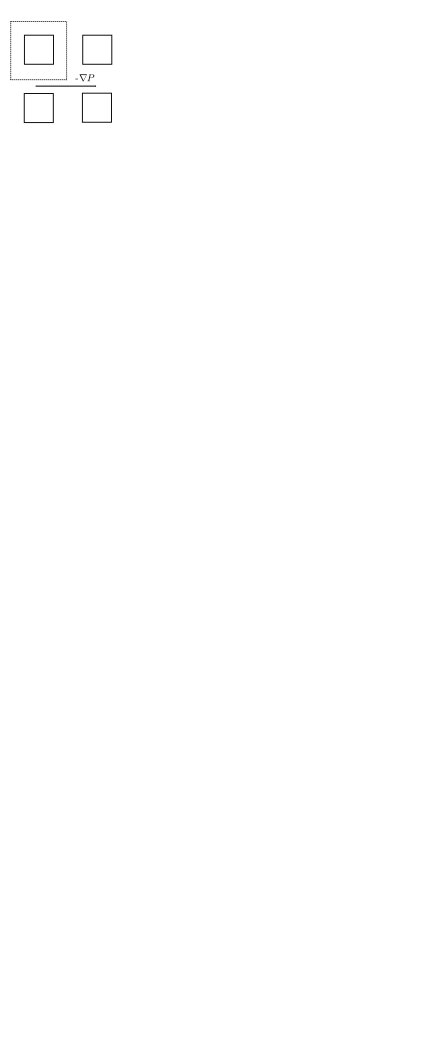
\includegraphics[width=0.35\textwidth]{fig/square_setup.pdf}}
  \caption[Sketch of setups for two physical 2D systems.]{Sketch of
    setups for the two physical 2D systems that are modelled. In (a),
    electroosmotic flow through a channel with heterogenously charged
    walls. In (b), pressure driven flow in an array of squares.}
  \label{fig:res:setup}
\end{figure}

The resulting velocity profile together with the charge distribution
of positive ions in the steady state is presented in
fig. \ref{fig:res:hetro}.

\begin{figure}
  \centering
  \subfloat[Velocity field
    ]{\label{fig:res:ta1}\includegraphics[width=0.32\textwidth]{fig/field_hetro.pdf}}      
  \hspace{5pt} \subfloat[$|\ubf|$
  ]{\label{fig:res:ts2}\includegraphics[width=0.32\textwidth]{fig/u_hetro.pdf}}  
\hspace{5pt} \subfloat[$\C_+$
  ]{\label{fig:res:t2}\includegraphics[width=0.32\textwidth]{fig/c_hetro.pdf}}
  \caption[Velocity field for flow in channel with heterogeneously
    charged walls.]{Visualised velocity field (a), magnitude of the
    velocities (b) and charge concentration of positive ions for a
    flow in a 2D channel with heterogeneously charged walls. A
    constant electric field of 50 kV/m drives the flow. The velocity
    field in (b) varies from $0.02 \mu$m/s (blue) to $2.2 \mu$m/s
    (red). The charge concentration in (c) varies from $0.45\C_0 $
    (blue) to $2.12\C_0$ (red).}
  \label{fig:res:hetro}
\end{figure}

There is an accumulation of positive and negative ions in the vicinity
of the negative and positive charged boundaries respectively. In the
middle of the channel, the fluid is neutral.

The vortexes obtained agrees qualitatively with those computed in
\cite{lbm-wang}. This kind of system is for example used in mixing of
charge fluids \cite{mixing}. Varying charges are imposed on the
boundary of a domain and an electric field is applied, this results
typically in a flow similar to the vortexes obtained here.



\section{Flow in an array of charged squares}

In this section, flow through a periodic structure is modelled. The
structure is consists of squares placed in a periodic pattern shown in
fig. \ref{fig:res:square}. The unit cell, used in the computation is
marked by the dashed box in the figure. The dimension of the unit cell
is chosen to $10 \mu$m and the permeability through the structure is
investigated for different sizes of the squares. Also the effect of
having charged vs. uncharged squares is studied. 

In fig. \ref{fig:res:s_uncharged} and fig. \ref{fig:res:s_charged} the
computed velocity fields around a square in a unit cell is
visualised. The side of the square is of length $0.5d$.   

\begin{figure}
  \centering
  \subfloat[Velocity field
    ]{\label{fig:res:hetasdro}\includegraphics[width=0.47\textwidth]{fig/s_field_uncharged.pdf}}      
  \hspace{5pt} \subfloat[$|\ubf|$
  ]{\label{fig:res:squasadre}\includegraphics[width=0.47\textwidth]{fig/s_u_uncharged.pdf}}
  \caption[Velocity field for flow through an array of
    uncharged squares.]{Visualised velocity field for flow
    through an array of \textbf{uncharged} squares. The magnitude of
    the velocity varies between 0.20 m/s (red) to 0 m/s (blue).}
  \label{fig:res:s_uncharged}
\end{figure}


\begin{figure}
  \centering
  \subfloat[Velocity field
    ]{\label{fig:res:asas}\includegraphics[width=0.47\textwidth]{fig/s_field_charged.pdf}}      
  \hspace{5pt} \subfloat[$|\ubf|$
  ]{\label{fig:res:asdda}\includegraphics[width=0.47\textwidth]{fig/s_u_charged.pdf}}
  \caption[Velocity field for flow through an array of charged
    squares.]{Visualised velocity field for flow through an array of
    \textbf{charged} squares. The magnitude of the velocity varies
    between 0.16 m/s (orange) to 0 m/s (blue). The surface charge is
    set to $\sigma_s = 1.78 \mu$C/m$^2$. The same colour scale as is
  fig. \ref{fig:res:s_uncharged} is used.}
  \label{fig:res:s_charged}
\end{figure}

The main effect noted that the charge on the square has on the flow,
is that it is slowed down. This is due to that charge inhomogeneities
arise when the charged square is introduced and from this the flow is
slowed down due to the electroviscous effect. In
figs. \ref{fig:res:mid} and \ref{fig:res:pre}, the velocity component
in the pressure drop direction (x) is shown in a section at $x = d/2$
and $x = 0$ respectively.  

\begin{figure}
\begin{center}
\includegraphics[width=0.9\textwidth]{fig/square_u_mid.pdf}
\end{center}
\caption[Section of the velocity field through a square
  array.]{Velocity profiles across the square array at $x = d/2$ in
  the cell. The sides of the squares are varied between $0.3d$, $0.5d$
  and $0.7d$ where $d = 10 \mu$m is the length of the cell. The flow
  is driven by a pressure gradient and the uncharged (dashed) and
  charged (solid) squares are compared. $\sigma_s = 1.78 \mu$C/m$^2$
  (solid), $\partial_xP = 0.5$ kPa/m and $u_0 = 1$ mm/s. }
\label{fig:res:mid}
\end{figure}

\begin{figure}
\begin{center}
\includegraphics[width=0.9\textwidth]{fig/square_pre_u.pdf}
\end{center}
\caption[Section of the velocity field through a square
  array.]{Velocity profiles across the square array at $x = 0$ in the
  cell. The sides of the squares are varied between $0.3d$, $0.5d$ and
  $0.7d$ where $d = 10 \mu$m is the length of the cell. The flow is
  driven by a pressure gradient and the uncharged (dashed) and charged
  (solid) squares are compared. $\sigma_s = 1.78 \mu$C/m$^2$ (solid),
  $\partial_xP = 0.5$ kPa/m and $u_0 = 1$ mm/s. }
\label{fig:res:pre}
\end{figure}

